% Options for packages loaded elsewhere
\PassOptionsToPackage{unicode}{hyperref}
\PassOptionsToPackage{hyphens}{url}
%
\documentclass[
]{article}
\usepackage{amsmath,amssymb}
\usepackage{lmodern}
\usepackage{iftex}
\ifPDFTeX
  \usepackage[T1]{fontenc}
  \usepackage[utf8]{inputenc}
  \usepackage{textcomp} % provide euro and other symbols
\else % if luatex or xetex
  \usepackage{unicode-math}
  \defaultfontfeatures{Scale=MatchLowercase}
  \defaultfontfeatures[\rmfamily]{Ligatures=TeX,Scale=1}
\fi
% Use upquote if available, for straight quotes in verbatim environments
\IfFileExists{upquote.sty}{\usepackage{upquote}}{}
\IfFileExists{microtype.sty}{% use microtype if available
  \usepackage[]{microtype}
  \UseMicrotypeSet[protrusion]{basicmath} % disable protrusion for tt fonts
}{}
\makeatletter
\@ifundefined{KOMAClassName}{% if non-KOMA class
  \IfFileExists{parskip.sty}{%
    \usepackage{parskip}
  }{% else
    \setlength{\parindent}{0pt}
    \setlength{\parskip}{6pt plus 2pt minus 1pt}}
}{% if KOMA class
  \KOMAoptions{parskip=half}}
\makeatother
\usepackage{xcolor}
\usepackage[margin=1in]{geometry}
\usepackage{color}
\usepackage{fancyvrb}
\newcommand{\VerbBar}{|}
\newcommand{\VERB}{\Verb[commandchars=\\\{\}]}
\DefineVerbatimEnvironment{Highlighting}{Verbatim}{commandchars=\\\{\}}
% Add ',fontsize=\small' for more characters per line
\usepackage{framed}
\definecolor{shadecolor}{RGB}{248,248,248}
\newenvironment{Shaded}{\begin{snugshade}}{\end{snugshade}}
\newcommand{\AlertTok}[1]{\textcolor[rgb]{0.94,0.16,0.16}{#1}}
\newcommand{\AnnotationTok}[1]{\textcolor[rgb]{0.56,0.35,0.01}{\textbf{\textit{#1}}}}
\newcommand{\AttributeTok}[1]{\textcolor[rgb]{0.77,0.63,0.00}{#1}}
\newcommand{\BaseNTok}[1]{\textcolor[rgb]{0.00,0.00,0.81}{#1}}
\newcommand{\BuiltInTok}[1]{#1}
\newcommand{\CharTok}[1]{\textcolor[rgb]{0.31,0.60,0.02}{#1}}
\newcommand{\CommentTok}[1]{\textcolor[rgb]{0.56,0.35,0.01}{\textit{#1}}}
\newcommand{\CommentVarTok}[1]{\textcolor[rgb]{0.56,0.35,0.01}{\textbf{\textit{#1}}}}
\newcommand{\ConstantTok}[1]{\textcolor[rgb]{0.00,0.00,0.00}{#1}}
\newcommand{\ControlFlowTok}[1]{\textcolor[rgb]{0.13,0.29,0.53}{\textbf{#1}}}
\newcommand{\DataTypeTok}[1]{\textcolor[rgb]{0.13,0.29,0.53}{#1}}
\newcommand{\DecValTok}[1]{\textcolor[rgb]{0.00,0.00,0.81}{#1}}
\newcommand{\DocumentationTok}[1]{\textcolor[rgb]{0.56,0.35,0.01}{\textbf{\textit{#1}}}}
\newcommand{\ErrorTok}[1]{\textcolor[rgb]{0.64,0.00,0.00}{\textbf{#1}}}
\newcommand{\ExtensionTok}[1]{#1}
\newcommand{\FloatTok}[1]{\textcolor[rgb]{0.00,0.00,0.81}{#1}}
\newcommand{\FunctionTok}[1]{\textcolor[rgb]{0.00,0.00,0.00}{#1}}
\newcommand{\ImportTok}[1]{#1}
\newcommand{\InformationTok}[1]{\textcolor[rgb]{0.56,0.35,0.01}{\textbf{\textit{#1}}}}
\newcommand{\KeywordTok}[1]{\textcolor[rgb]{0.13,0.29,0.53}{\textbf{#1}}}
\newcommand{\NormalTok}[1]{#1}
\newcommand{\OperatorTok}[1]{\textcolor[rgb]{0.81,0.36,0.00}{\textbf{#1}}}
\newcommand{\OtherTok}[1]{\textcolor[rgb]{0.56,0.35,0.01}{#1}}
\newcommand{\PreprocessorTok}[1]{\textcolor[rgb]{0.56,0.35,0.01}{\textit{#1}}}
\newcommand{\RegionMarkerTok}[1]{#1}
\newcommand{\SpecialCharTok}[1]{\textcolor[rgb]{0.00,0.00,0.00}{#1}}
\newcommand{\SpecialStringTok}[1]{\textcolor[rgb]{0.31,0.60,0.02}{#1}}
\newcommand{\StringTok}[1]{\textcolor[rgb]{0.31,0.60,0.02}{#1}}
\newcommand{\VariableTok}[1]{\textcolor[rgb]{0.00,0.00,0.00}{#1}}
\newcommand{\VerbatimStringTok}[1]{\textcolor[rgb]{0.31,0.60,0.02}{#1}}
\newcommand{\WarningTok}[1]{\textcolor[rgb]{0.56,0.35,0.01}{\textbf{\textit{#1}}}}
\usepackage{longtable,booktabs,array}
\usepackage{calc} % for calculating minipage widths
% Correct order of tables after \paragraph or \subparagraph
\usepackage{etoolbox}
\makeatletter
\patchcmd\longtable{\par}{\if@noskipsec\mbox{}\fi\par}{}{}
\makeatother
% Allow footnotes in longtable head/foot
\IfFileExists{footnotehyper.sty}{\usepackage{footnotehyper}}{\usepackage{footnote}}
\makesavenoteenv{longtable}
\usepackage{graphicx}
\makeatletter
\def\maxwidth{\ifdim\Gin@nat@width>\linewidth\linewidth\else\Gin@nat@width\fi}
\def\maxheight{\ifdim\Gin@nat@height>\textheight\textheight\else\Gin@nat@height\fi}
\makeatother
% Scale images if necessary, so that they will not overflow the page
% margins by default, and it is still possible to overwrite the defaults
% using explicit options in \includegraphics[width, height, ...]{}
\setkeys{Gin}{width=\maxwidth,height=\maxheight,keepaspectratio}
% Set default figure placement to htbp
\makeatletter
\def\fps@figure{htbp}
\makeatother
\setlength{\emergencystretch}{3em} % prevent overfull lines
\providecommand{\tightlist}{%
  \setlength{\itemsep}{0pt}\setlength{\parskip}{0pt}}
\setcounter{secnumdepth}{-\maxdimen} % remove section numbering
\ifLuaTeX
  \usepackage{selnolig}  % disable illegal ligatures
\fi
\IfFileExists{bookmark.sty}{\usepackage{bookmark}}{\usepackage{hyperref}}
\IfFileExists{xurl.sty}{\usepackage{xurl}}{} % add URL line breaks if available
\urlstyle{same} % disable monospaced font for URLs
\hypersetup{
  pdftitle={Hausaufgabe 1},
  pdfauthor={Team 4 (Milena Mensching, Justus Weyers)},
  hidelinks,
  pdfcreator={LaTeX via pandoc}}

\title{Hausaufgabe 1}
\author{Team 4 (Milena Mensching, Justus Weyers)}
\date{2022-11-03}


\begin{document}
\maketitle

\hypertarget{aufgabe-1}{%
\section{Aufgabe 1}\label{aufgabe-1}}
\textbf{Die Periodendauer eines Pendels wird gemessen. 
Ihr Wert wird mit \((10,0 \pm 0,1)s\) angegeben. 
Wie groß ist die relative Messunsicherheit?}

\begin{equation}\label{eq:uRel}
  \begin{split}
    u_{rel} &= \frac{u_x}{x} \\
    \Rightarrow \vert\frac{\pm0,1s}{10,0s}\vert & = 0,01 = 1\%.
  \end{split}
\end{equation}

\begin{itemize}
  \item  $u_{rel}$: Relative Messunsicherheit
  \item  $u_x$: Absolute Messunsicherheit
  \item  $x$: Bestwert
\end{itemize}

\hypertarget{aufgabe-2}{%
\section{Aufgabe 2:}\label{aufgabe-2}}

\textbf{Es wurde eine Geschwindigkeit von \(6 \frac{km}{h}\) mit einer relativen Unsicherheit von \(1 \%\) gemessen. 
Wie groß ist die absolute Messunsicherheit?}

Aus Gleichung \ref{eq:uRel} folgt durch Umstellen:
\begin{equation}\label{eq:uAbs}
  \begin{split}
  	u_x &= u_{rel}*x \\
    \Rightarrow & = \pm 0,01 * 6 \frac{km}{h}\\
    &= \pm 0,06 \frac{km}{h}.\\
  \end{split}
\end{equation}

\hypertarget{aufgabe-3}{%
\section{Aufgabe 3}\label{aufgabe-3}}
\textbf{Ein analoger Spannungsmesser hat die Güteklasse 2 (d.h. die Messunsicherheit beträgt \(2 \%\) des Messbereichs-Endwertes). 
Wie groß ist die relative Messunsicherheit der Anzeige, wenn im \(10 V\)-Messbereich \(2,00 V\) abgelesen werden?}

Das Gerät entspricht der Güteklasse 2. 
Daraus folgt, dass die Messunsicherheit bei einem Vollausschlag von \(10 V\) bei \(\pm0,2 V\) liegt. 
Mit Gleichung\ref{eq:uRel} ergibt sich:

\begin{center}
$\vert\frac{\pm 0,2V}{2V}\vert = 0,01 = 1\%$.
\end{center}

\hypertarget{aufgabe-4}{%
\section{Aufgabe 4:}\label{aufgabe-4}}

\textbf{Sie wiegen in der Küche mit einer digitalen elektronischen Waage dessen kleinste Schrittweite (auch Auflösung genannt) \(0,1 g\) beträgt einen Apfel. 
Der Apfel wiegt laut Anzeige \(120,0 g\). 
Wie groß ist die gesamte Messunsicherheit der Messung, wenn der Gerätehersteller eine Gerätemessunsicherheit von \(1\%\) v. Messwert + \(2 [dgt.]\) angibt?}

Berechnung der Skalenungenauigkeit \(u_{Skala}\). 
Der tatsächliche Wert kann zwischen \(119,95g\) und \(120,05g\) liegen (\(\rightarrow a=0,1g\)). Daraus folgt für \(u_{Skala}\) (digitale Waage):

\begin{equation}\label{eq:uDigit}
  \begin{split}
  	u_{Skala} &= \frac{a}{2\sqrt{3}}\\
    \Rightarrow &= \frac{0,1g}{2\sqrt{3}}\\
    &= \pm 0,058g.
  \end{split}
\end{equation}

\begin{itemize}
  \item $u_{Skala}$: Messunsicherheit Skala
  \item $a$: Fehlerintervall
\end{itemize}

Aus der Aufgabenstellung folgt für die Messungenauigkeit der Waage \(u_{Gerät}\):

\begin{center}
  $u_{Gerät} = 0,01 * 120g + 2 [dgt.] = \pm 1,4g.$
\end{center}

Die Gesamtunsicherheit berechnet sich dann als:
\begin{equation}\label{eq:uGes}
  \begin{split}
    u_{Gesamt} &= \sqrt{u_{Skala}^2+u_{Gerät}^2}\\
    \Rightarrow &= \sqrt{(\pm0,058g)^2\pm(1,4g)^2}\\
    &= \pm 1,4g.
  \end{split}
\end{equation}

\hypertarget{aufgabe-5}{%
\section{Aufgabe 5:}\label{aufgabe-5}}

\textbf{Eine Spannung wurde gleichzeitig mit zwei baugleichen Analog-Multimetern (AMM) genau einmal gemessen: Messbereich: \(200 mV\), Garantiefehlergrenze: \(\pm (0,5\% v. Messwert. + 0,1\% v. Messbereich)\); Messwert 1 (AMM1): \(22,0 mV\), Messwert 2 (AMM2): \(22,5 mV\) (\(\rightarrow a=0,1g\)). 
Geben Sie die beiden Messergebnisse zusammen mit der Standardmessunsicherheit in korrekter Schreibweise an.}

AMM1:

Fehler \(0,5\%\) vom Messwert:
\(u_{Messwert} = 0,005 * 22,0mV = \pm0,11mV\).

Fehler \(0,1\%\) vom Messbereich:
\(u_{Messbereich} = 0,001 * 200mV = \pm0,20mV\).

Fehler der analogen Skala:
\(u_{Skala} = \frac{a}{2\sqrt{6}} = \frac{0,1mV}{2\sqrt{6}}=\pm0,020mV\).

Gesamtfehler errechnet sich als: 
\begin{equation}\label{eq:uGesSMM}
  	\begin{split}
		u_{Gesamt} &= \sqrt{u_{Skala}^2+u_{Messwert}^2+u_{Messbereich}^2}\\
        &= \sqrt{(\pm 0,020)^2+(\pm 0,11)^2+(\pm0,20)^2}mV\\
        &= \pm 0,23mV
	\end{split}
\end{equation}

Gerätunsicherheit:
\(u_{AMM1} = \sqrt{u_{Messwert}^2+u_{Messbereich}^2} = \pm0,23 mV\).

AMM2:

Fehler \(0,5\%\) vom Messwert:
\(u_{Messwert} = 0,005 * 22,5mV \approx \pm 0,11mV\).

Fehler \(0,1\%\) vom Messbereich:
\(u_{Messbereich} = 0,001 * 200mV = \pm0,20mV\).

Fehler der analogen Skala:
\(u_{Skala} = \frac{a}{2\sqrt{6}} = \frac{0,1mV}{2\sqrt{6}}=\pm0,020mV\).

Gesamtfehler errechnet sich als analog zu Gleichung \ref{eq:uGesSMM}:
\begin{align*}
	\begin{split}
		u_{Gesamt}&= \sqrt{(\pm 0,020)^2+(\pm 0,11)^2+(\pm0,20)^2}mV\\
        &= \pm 0,23mV
	\end{split}
\end{align*}

Gerätunsicherheit:
\(u_{AMM2} = \sqrt{u_{Messwert}^2+u_{Messbereich}^2} = \pm0,23 mV\).

\hypertarget{aufgabe-6}{%
\section{Aufgabe 6:}\label{aufgabe-6}}

\textbf{Nehmen Sie nun an, Sie ändern den Messbereich des Multimeters und damit die Garantiefehlergrenze des Multimeters auf \(\pm(0,2\% v. Messwert. + 0,02\% vom Messbereich)\) für den Messbereich von \(2 V\). 
Es wird erneut gemessen - neuer Wert: \(20 mV\) (wobei im \(2V\) Messbereich, die kleinste ablesebare Skalenstrich ist \(10mV\)).
Ändert sich die Messunsicherheit des Messgerätes? 
Wie ändert sich die Messunsicherheit der Ableseskala?}

Fehler \(0,2\%\) vom Messwert:
\(u_{Messwert} = 0,002 * 20mV = \pm 0,04mV\).

Fehler \(0,02\%\) vom Messbereich:
\(u_{Messbereich} = 0,0002 * 2000mV = \pm0,4mV\).

Fehler der analogen Skala:
\(u_{Skala} = \frac{a}{2\sqrt{6}} = \frac{10mV}{2\sqrt{6}}=\pm2,0mV\).

Messunsicherheit des Multimeters: 
\begin{align*}
	\begin{split}
    	u_{Gerät} &= \sqrt{u_{Messwert}^2+u_{Messbereich}^2}\\
    	\Rightarrow  &= \sqrt{(\pm 0,04)^2+(\pm 0,4)^2}\\
        &= \pm 0,4mV.
  \end{split}
\end{align*}

Der Betrag der Messunsicherheit des Multimeters verdoppelt sich mit \(\pm 0,4mV\) im Vergleich zu den Gerätmessunsicherheiten aus Aufgabe 5, welche für beide Geräte \(\pm 0,23mV\) betrug.

Der Fehler der Ableseskala steigt in diesem Vergleich hingegen um zwei
Größenordnungen von \(\pm 0,020mV\) in Aufgabe 5 auf \(\pm 2,0mV\) in
Aufgabe 6.

\hypertarget{aufgabe-7}{%
\section{Aufgabe 7:}\label{aufgabe-7}}

\textbf{Die Temperatur eines Kühlschranks wurde mehrmals gemessen. 
Es wurde diese Messreihe aufgenommen:}

\begin{longtable}[]{@{}llllllll@{}}
	\toprule()
	\endhead
	T (°C) & 7,6 & 7,8 & 8,2 & 7,7 & 7,8 & 8,3 & 8,0 \\
	\bottomrule()
\end{longtable}

\newpage

\textbf{Geben Sie den Bestwert für T zusammen mit der Messunsicherheit (Typ A) in korrekter Schreibweise an.}

Es finden folgende Formeln für die Berechnung von Statistik- und
Fehlerkenngrößen Verwendung:

\begin{itemize}
	\tightlist
	\item  Mittelwert \(\bar{x} = \frac{1}{n}\sum\limits_{i}^{n}x_i\)
	\item  Standardabweichung  \(\sigma = \sqrt{\frac{1}{n-1}\sum\limits_{i}^{n}(x_i-\bar{x})^2)}\)
	\item  Standardabweichung des Mittelwertes \(\sigma_{\bar{x}} = \frac{\sigma}{\sqrt{n}}\)
	\item  Vertrauensabweichung \(\varepsilon = t*\sigma_{\bar{x}}\)
\end{itemize}

Mit \(n\): Anzahl der (Mess)Werte, \(x_i\): \(i\)-ter Messwert, \(t\): Student Faktor, hier \(1,08\).
Die Berechnung erfolgt durch Einabe in R:

\begin{Shaded}
\begin{Highlighting}[]
\CommentTok{\# Eingabe der Messwerte}
\NormalTok{temp\_messwerte }\OtherTok{\textless{}{-}} \FunctionTok{c}\NormalTok{(}\FloatTok{7.6}\NormalTok{,}\FloatTok{7.8}\NormalTok{,}\FloatTok{8.2}\NormalTok{,}\FloatTok{7.7}\NormalTok{,}\FloatTok{7.8}\NormalTok{,}\FloatTok{8.3}\NormalTok{,}\FloatTok{8.0}\NormalTok{)}

\CommentTok{\# Berechnung Mittelwert}
\NormalTok{Mittelwert }\OtherTok{\textless{}{-}} \FunctionTok{mean}\NormalTok{(temp\_messwerte)}

\CommentTok{\# Berechnung Standardabweichung (SD)}
\NormalTok{SD }\OtherTok{=} \FunctionTok{sd}\NormalTok{(temp\_messwerte)}

\CommentTok{\# Berechnung Standardabweichung des Mittelwertes (SDM)}
\NormalTok{SDM }\OtherTok{=}\NormalTok{ SD}\SpecialCharTok{/}\FunctionTok{sqrt}\NormalTok{(}\FunctionTok{length}\NormalTok{(temp\_messwerte))}

\CommentTok{\# Student T{-}Faktor für n = 7}
\NormalTok{t }\OtherTok{=} \FloatTok{1.08}

\CommentTok{\# Berechnung Vertrauensabweichung (VAB)}
\NormalTok{VAB }\OtherTok{=}\NormalTok{ t}\SpecialCharTok{*}\NormalTok{SDM}

\CommentTok{\# Ausgabe der errechneten Werte als Dataframe}
\FunctionTok{data.frame}\NormalTok{(Maßzahl }\OtherTok{=} \FunctionTok{c}\NormalTok{(}\StringTok{\textquotesingle{}Mittelwert\textquotesingle{}}\NormalTok{, }\StringTok{\textquotesingle{}Standardabweichung\textquotesingle{}}\NormalTok{,}
                       \StringTok{\textquotesingle{}Standardabweichung des Mittelwertes\textquotesingle{}}\NormalTok{,}
                       \StringTok{\textquotesingle{}t{-}Faktor\textquotesingle{}}\NormalTok{, }\StringTok{\textquotesingle{}Vertrauensabweichung\textquotesingle{}}\NormalTok{),}
           \AttributeTok{Werte =} \FunctionTok{round}\NormalTok{(}\FunctionTok{c}\NormalTok{(Mittelwert, SD, SDM, t, VAB), }\DecValTok{4}\NormalTok{))}
\end{Highlighting}
\end{Shaded}

\begin{verbatim}
##                               Maßzahl  Werte
## 1                          Mittelwert 7.9143
## 2                  Standardabweichung 0.2610
## 3 Standardabweichung des Mittelwertes 0.0986
## 4                            t-Faktor 1.0800
## 5                Vertrauensabweichung 0.1065
\end{verbatim}

Für die Messunsicherheit ergibt sich daraus:
\(u = (7,91 \pm 0,11)\)°\(C\).

\newpage

\hypertarget{aufgabe-8}{%
\section{Aufgabe 8:}\label{aufgabe-8}}

\textbf{Geben Sie die folgenden Messergebnisse korrekt an:}

\begin{longtable}[]{@{}
  >{\raggedright\arraybackslash}p{(\columnwidth - 2\tabcolsep) * \real{0.5213}}
  >{\raggedright\arraybackslash}p{(\columnwidth - 2\tabcolsep) * \real{0.4787}}@{}}
	\toprule()
	\begin{minipage}[b]{\linewidth}\raggedright
		Inkorrekt
	\end{minipage} & \begin{minipage}[b]{\linewidth}\raggedright
		Hoffentlich korrekt
	\end{minipage} \\
	\midrule()
	\endhead
	\(a=(9,82\pm0,02385)\frac{m}{s^2}\) &
	\(a=(9,820\pm0,024)\frac{m}{s^2}\) \\
	\(Q=(0,1562*10^{-15}\pm 689,76*10^{-19})C\) &
	\(Q=(0,1560*10^{-15}\pm690*10^{-19})C\) \\
	\(v=(199798673,67\pm 7245,98132)\frac{m}{s}\) &
	\(v=(199798700\pm7200)\frac{m}{s}\) \\
	\(\lambda=(885,589*10^{-11}\pm 0,004985*10^{-8})m\) &
	\(\lambda=(0,8856*10^{-8}\pm 0,0050*10^{-8})m\) \\
	\(U=1,81kV, u(U)=1693mV\) & \(U=(1810,0\pm 1,7)V\) \\
	\bottomrule()
\end{longtable}

\hypertarget{aufgabe-9}{%
\section{Aufgabe 9:}\label{aufgabe-9}}
\textbf{Lesen Sie die folgenden Messgrößen so gut wie möglich ab und geben Sie sie korrekt an!} 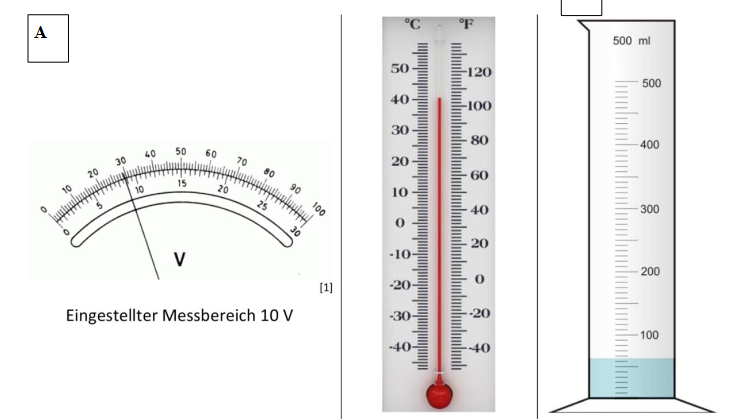
\includegraphics{A9.png}

\hypertarget{a-voltmeter}{%
\subsection{a) Voltmeter}\label{a-voltmeter}}

Skalenart: Analog

Abgelesener Bestwert: \(8,9 V\)

Kleinstes ablesbare Intervall \(a\): \(0,5V\)

Da es sich bei der Anzeige des Voltmeters um eine analoge Anzeige handelt wird für die Berechnung der Messunsicherheit der Ableseskala \(u_{skala}\) die Formel \(u_{skala}=\frac{a}{2\sqrt{6}}\) verwendet:
\[\Rightarrow u_{skala} = \pm\frac{0,5V}{2\sqrt{6}} = \pm 0,10V\]. 
Damit ergibt sich das Messergebnis zu: \((8,9\pm0,10)V\).

\hypertarget{b-thermometer}{%
\subsection{b) Thermometer}\label{b-thermometer}}

Skalenart: Analog

Abgelesener Bestwert: \(41^\circ\text{C}\)

Kleinstes ablesbares Intervall \(a\): \(1^\circ\text{C}\)

Da es sich bei der Anzeige des Thermometers um eine analoge Anzeige handelt wird für die Berechnung der Messunsicherheit der Ableseskala \(u_{skala}\) die Formel \(u_{skala}=\frac{a}{2\sqrt{6}}\) verwendet: \[\Rightarrow u_{skala} = \pm\frac{1^\circ\text{C}}{2\sqrt{6}} = \pm 0,20^\circ\text{C}\].
Damit ergibt sich das Messergebnis zu: \((41,00\pm0,20)^\circ\text{C}\).

\hypertarget{c-standzylinder}{%
\subsection{c) Standzylinder}\label{c-standzylinder}}

Skalenart: Analog

Abgelesener Bestwert:
\((\frac{1}{2}+\frac{3}{24})*100ml = \frac{15}{24}*100ml= 62,5ml\)

Kleinstes ablesbares Intervall \(a\): \(\frac{1}{12}*100ml\)

Der Standzylinder besitzt eine analoge Skala. 
Für die Berechnung der Messunsicherheit der Ableseskala \(u_{skala}\) findet die Formel \(u_{skala}=\frac{a}{2\sqrt{6}}\) Verwendung: \[\Rightarrow u_{skala} = \pm\frac{\frac{1}{12}*100ml}{2\sqrt{6}} = \pm 1,7ml\]
Damit ergibt sich das Messergebnis zu: \((62,5\pm1,7)ml\).

\end{document}
